\documentclass[11pt,a4paper]{article}

% =====================================================================
% PACKAGES
% =====================================================================
\usepackage[utf8]{inputenc}
\usepackage[T1]{fontenc}
\usepackage{lmodern}
\usepackage[margin=1in]{geometry}
\usepackage{amsmath,amssymb,amsfonts}
\usepackage{graphicx}
\usepackage{booktabs}
\usepackage{multirow}
\usepackage{array}
\usepackage{tabularx}
\usepackage[table]{xcolor}
\usepackage{microtype}
\usepackage{caption}
\usepackage{enumitem}
\usepackage{fancyhdr}
\usepackage{titlesec}
\usepackage[most]{tcolorbox}
\usepackage{tikz}
\usetikzlibrary{arrows.meta, positioning, calc}
\usepackage{cite}
\usepackage{hyperref}

% =====================================================================
% COLOURS
% =====================================================================
\definecolor{navy}{HTML}{1F3A5F}
\definecolor{accent}{HTML}{1B7F9E}
\definecolor{softblue}{HTML}{EAF3F8}
\definecolor{softgreen}{HTML}{E8F5E9}
\definecolor{softgray}{HTML}{F4F5F7}
\definecolor{champion}{HTML}{DDF1E4}

\hypersetup{
    colorlinks=true,
    linkcolor=navy,
    citecolor=accent,
    urlcolor=accent,
    pdftitle={HinglishPulse: Sentiment Analysis for Code-Mixed Social Media Text},
    pdfauthor={Suraj, Subhadeep Das, Aayush Kumar, Sudeshna Kumari}
}

% =====================================================================
% LAYOUT & STYLE
% =====================================================================
\setlength{\parskip}{0.5em}
\setlength{\parindent}{0pt}
\renewcommand{\arraystretch}{1.18}
\setlist{itemsep=0.2em, topsep=0.3em}
\captionsetup{font=small, labelfont={bf,color=navy}, skip=6pt}

\titleformat{\section}{\Large\bfseries\color{navy}}{\thesection}{0.7em}{}[\vspace{0.45em}{\color{navy}\titlerule[0.8pt]}]
\titleformat{\subsection}{\large\bfseries\color{accent}}{\thesubsection}{0.6em}{}
\titlespacing*{\section}{0pt}{1.6em}{0.9em}

\pagestyle{fancy}
\fancyhf{}
\fancyhead[L]{\small\color{gray}HinglishPulse -- Technical Report}
\fancyhead[R]{\small\color{gray}SemEval-2020 Task 9}
\fancyfoot[C]{\small\thepage}
\renewcommand{\headrulewidth}{0.3pt}

% Callout box: \begin{keybox}{Title} ... \end{keybox}
\newtcolorbox{keybox}[1]{
    enhanced, breakable, colback=softblue, colframe=accent,
    fonttitle=\bfseries, title={#1}, boxrule=0.6pt, arc=2pt,
    left=8pt, right=8pt, top=5pt, bottom=5pt
}

% Figure that falls back to a labelled placeholder if the image is missing
\newcommand{\safefig}[2]{%
    \IfFileExists{#1}%
      {\includegraphics[width=#2\textwidth]{#1}}%
      {\fcolorbox{gray!50}{softgray}{\parbox[c][4.5cm][c]{#2\textwidth}{\centering\small\color{gray}%
        Figure placeholder\\[2pt]\texttt{\detokenize{#1}}}}}%
}

% =====================================================================
% TITLE BLOCK
% =====================================================================
\newcommand{\memberid}{12340040}

\begin{document}

\begin{center}
    {\color{navy}\rule{\textwidth}{1.2pt}}\\[1.2em]
    {\Huge\bfseries\color{navy} HinglishPulse}\\[0.5em]
    {\LARGE\bfseries End-to-End Sentiment Analysis and Intelligence Platform for Code-Mixed Social Media Text}\\[0.8em]
    {\large An Empirical Study and Full-Stack Implementation on SemEval-2020 Task 9}\\[1.2em]
    {\color{navy}\rule{\textwidth}{0.5pt}}\\[1.4em]

    {\large\bfseries Project Team}\\[0.6em]
    \begin{tabular}{@{}lc@{}}
        \toprule
        \textbf{Member Name} & \textbf{ID No.} \\
        \midrule
        Suraj           & \memberid \\
        Subhadeep Das   & \memberid \\
        Aayush Kumar    & \memberid \\
        Sudeshna Kumari & \memberid \\
        \bottomrule
    \end{tabular}\\[1.4em]
    {\normalsize Research \& Engineering Technical Report \quad$\cdot$\quad November 2026}
\end{center}

\vspace{0.8em}

\begin{abstract}
\noindent
\textit{Hinglish} --- Hindi and English mixed together and typed in the Latin alphabet --- is the everyday language of millions of social media users, yet it is hard for machines to read: spellings are not standardised, grammar switches mid-sentence, and many words in new text have never been seen before. In this project we build \textbf{HinglishPulse}, a complete and reproducible system that classifies the sentiment (negative, neutral, positive) of Hinglish tweets using the official SemEval-2020 Task 9 (SentiMix) dataset of 20,594 tweets.

We (i) design a text-cleaning and spelling-normalisation pipeline for Romanised Hindi, (ii) build subword features with FastText, and (iii) compare a classical TF-IDF + Logistic Regression baseline against four neural networks: LSTM, BiLSTM, 1D CNN, and a hybrid BiLSTM+Conv1D. The hybrid model performs best, reaching a validation accuracy of \textbf{91.57\%} and a Macro F1-score of \textbf{91.64\%}, compared with 87.10\% and 87.12\% for the baseline. Finally, we deploy the model behind a \textbf{FastAPI} inference service and a dark-themed \textbf{React + TypeScript} dashboard, with hash-verified data hand-offs so that every result can be reproduced.
\end{abstract}

\noindent\textbf{Keywords:} Hinglish, code-mixed sentiment analysis, SemEval-2020 Task 9, BiLSTM-CNN, FastText, FastAPI, React.

\begin{keybox}{Project at a Glance}
\small
\begin{tabularx}{\textwidth}{@{}lX@{}}
\textbf{Problem}   & Classify the sentiment of code-mixed Hinglish tweets into three classes. \\
\textbf{Data}      & SemEval-2020 Task 9: 20,594 tweets (14,594 train / 3,000 validation / 3,000 test). \\
\textbf{Challenge} & 30.25\% of test-set words never appear in the training set (out-of-vocabulary). \\
\textbf{Approach}  & Custom normalisation $\rightarrow$ FastText subword features $\rightarrow$ five models compared. \\
\textbf{Best model}& BiLSTM + Conv1D: 91.57\% accuracy, 91.64\% Macro F1 (validation). \\
\textbf{Deliverable}& FastAPI backend + React/TypeScript web dashboard with live inference. \\
\end{tabularx}
\end{keybox}

\newpage
{\setlength{\parskip}{0pt}\small\tableofcontents}
\newpage

% =====================================================================
\section{Introduction}
% =====================================================================

\subsection{Why Hinglish Is Difficult}
Code-mixing is the use of two or more languages within a single message. On platforms such as X (Twitter), Instagram, YouTube and WhatsApp, a very large number of users in South Asia write in \textit{Hinglish}: Hindi words, often with Hindi sentence structure, spelled phonetically in English letters. Typical difficulties are:

\begin{enumerate}
    \item \textbf{No standard spelling.} One Hindi word can be written many ways, e.g.\ \textit{nahin}, \textit{nahee}, \textit{nahein}, \textit{nahi} (all meaning ``not'').
    \item \textbf{Many unseen words.} Slang and creative spellings give an out-of-vocabulary (OOV) rate of over $30\%$ between training and test data.
    \item \textbf{Subtle meaning.} Sarcasm, implied negation (\textit{``kuch khaas nahi''}) and context-dependent polarity break simple bag-of-words assumptions.
\end{enumerate}

\subsection{What We Built}
\textbf{HinglishPulse} is a complete pipeline from raw tweets to a working web application. Our contributions are:
\begin{itemize}
    \item A \textbf{preprocessing and spelling-normalisation engine} designed for Romanised Hindi social media text.
    \item A \textbf{benchmark} of one classical model (TF-IDF + Logistic Regression) and four PyTorch networks (LSTM, BiLSTM, multi-kernel CNN, BiLSTM+Conv1D), with the best reaching a Macro F1 of $91.64\%$.
    \item A \textbf{full-stack deployment}: a FastAPI microservice and a React + TypeScript dashboard that lets users analyse text interactively and inspect model results.
\end{itemize}

\subsection{Overview of the Work}
Figure~\ref{fig:overview} summarises the six stages of the project; each is described in its own section.

\begin{figure}[htbp]
\centering
\resizebox{\textwidth}{!}{%
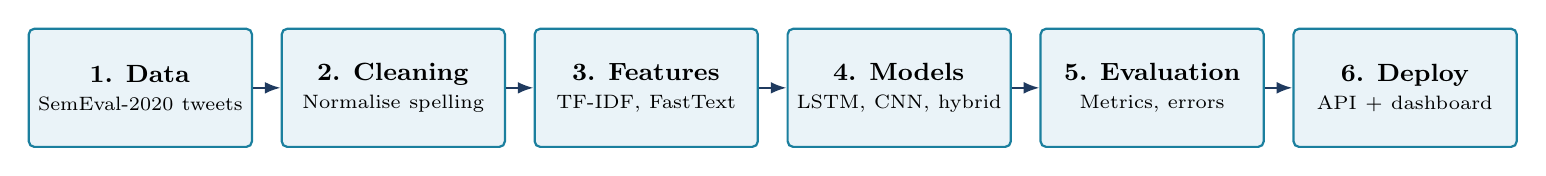
\begin{tikzpicture}[
    stage/.style={rectangle, rounded corners=2pt, draw=accent, fill=softblue, thick,
                  text width=2.6cm, align=center, minimum height=1.5cm, font=\small},
    arrow/.style={-{Latex[length=2mm]}, thick, draw=navy}
]
\node[stage] (a) {\textbf{1. Data}\\[-1pt]\scriptsize SemEval-2020 tweets};
\node[stage, right=0.35cm of a] (b) {\textbf{2. Cleaning}\\[-1pt]\scriptsize Normalise spelling};
\node[stage, right=0.35cm of b] (c) {\textbf{3. Features}\\[-1pt]\scriptsize TF-IDF, FastText};
\node[stage, right=0.35cm of c] (d) {\textbf{4. Models}\\[-1pt]\scriptsize LSTM, CNN, hybrid};
\node[stage, right=0.35cm of d] (e) {\textbf{5. Evaluation}\\[-1pt]\scriptsize Metrics, errors};
\node[stage, right=0.35cm of e] (f) {\textbf{6. Deploy}\\[-1pt]\scriptsize API + dashboard};
\foreach \s/\t in {a/b,b/c,c/d,d/e,e/f} \draw[arrow] (\s) -- (\t);
\end{tikzpicture}}
\caption{The six stages of the HinglishPulse project.}
\label{fig:overview}
\end{figure}

% =====================================================================
\section{Dataset and Data Engineering}
% =====================================================================

\subsection{SemEval-2020 Task 9 (SentiMix Hinglish)}
We use the official dataset from SemEval-2020 Task 9, \textit{Sentiment Analysis for Code-Mixed Social Media Text}~\cite{patwa2020semeval}. It contains $20{,}594$ tweets in three official partitions (Table~\ref{tab:dataset_splits}). Labels are encoded as Negative~$=0$, Neutral~$=1$, Positive~$=2$.

\begin{table}[htbp]
\centering
\small
\begin{tabular}{lcccc}
\toprule
\textbf{Split} & \textbf{Negative (0)} & \textbf{Neutral (1)} & \textbf{Positive (2)} & \textbf{Total Rows} \\
\midrule
Train       & 4,252 (29.1\%) & 5,473 (37.5\%) & 4,869 (33.4\%) & 14,594 \\
Validation  &   890 (29.7\%) & 1,128 (37.6\%) &   982 (32.7\%) &  3,000 \\
Test        &       ---      &       ---      &       ---      &  3,000 \\
\midrule
\textbf{Total} & \textbf{5,142} & \textbf{6,601} & \textbf{5,851} & \textbf{20,594} \\
\bottomrule
\end{tabular}
\caption{Class distribution across the official partitions. Test labels are not available to us, so class totals cover the 17,594 labelled rows (train + validation) while the total column counts all rows.}
\label{tab:dataset_splits}
\end{table}

The classes are only mildly imbalanced: Neutral is the largest ($37.5\%$), followed by Positive ($33.4\%$) and Negative ($29.1\%$). Because the test labels are unavailable, \textbf{all results in this report are measured on the validation split}.

\begin{figure}[htbp]
    \centering
    \safefig{figures/class_distribution.png}{0.7}
    \caption{Class balance across the training and validation splits.}
    \label{fig:class_dist}
\end{figure}

\subsection{Data Contracts and Leakage Prevention}
To keep results trustworthy and the software stable, we enforced the following rules:

\begin{itemize}
    \item \textbf{Fixed file schemas.} Every processed file has a strict column layout:
\end{itemize}
\begin{center}
\small
\begin{tabular}{ll}
\toprule
\textbf{File type} & \textbf{Columns} \\
\midrule
Split data  & \texttt{uid}, \texttt{text\_clean}, \texttt{label} \\
Predictions & \texttt{uid}, \texttt{y\_true}, \texttt{y\_pred}, \texttt{p\_neg}, \texttt{p\_neu}, \texttt{p\_pos} \\
\bottomrule
\end{tabular}
\end{center}
\begin{itemize}
    \item \textbf{No data leakage.} Vocabularies, tokenisers, the spelling lookup table, TF-IDF matrices and FastText weights were all fitted \textbf{only on the training split}, never on validation or test text.
    \item \textbf{Hash-verified hand-offs.} Two manifests (\texttt{H1\_MANIFEST.json} and \texttt{H2\_MANIFEST.json}) record SHA-256 checksums, row counts and column checks, so each stage can verify that it received exactly the files the previous stage produced.
\end{itemize}

% =====================================================================
\section{Exploratory Data Analysis}
% =====================================================================

\subsection{Sequence Lengths}
We measured tweet lengths to choose a padding/truncation length for the neural networks (Figure~\ref{fig:length_hist}).

\begin{figure}[htbp]
    \centering
    \safefig{figures/token_length_histogram.png}{0.75}
    \caption{Distribution of tokens per tweet in the training split.}
    \label{fig:length_hist}
\end{figure}

\begin{table}[htbp]
\centering
\small
\begin{tabular}{lc}
\toprule
\textbf{Statistic} & \textbf{Value (tokens)} \\
\midrule
Mean $\pm$ std.\ dev. & $18.42 \pm 9.14$ \\
Median                & 17 \\
95th percentile ($\tau_{95}$) & 35 \\
\bottomrule
\end{tabular}
\caption{Token-length statistics (training split).}
\end{table}

We therefore set $\text{max\_len}=35$ for all recurrent and convolutional models. This covers over $95\%$ of tweets without wasting computation on excessive padding.

\subsection{Out-of-Vocabulary Analysis}
The most important finding of the analysis is the large OOV rate:
\begin{itemize}
    \item Training vocabulary $\mathcal{V}_{\text{train}}$: $30{,}978$ unique tokens.
    \item Test vocabulary $\mathcal{V}_{\text{test}}$: $10{,}914$ unique tokens.
\end{itemize}
\begin{equation}
    \text{OOV Rate} = \frac{|\mathcal{V}_{\text{test}} \setminus \mathcal{V}_{\text{train}}|}{|\mathcal{V}_{\text{test}}|} = \mathbf{30.25\%}
\end{equation}
In other words, almost one in three distinct test words has never been seen during training, so a fixed word dictionary will fail on a large share of the input. This directly motivated our use of character n-grams and FastText subword embeddings (Section~\ref{sec:features}).

\subsection{Word Frequency (Zipf) Analysis}
The most frequent tokens are Romanised Hindi function words such as \textit{hai} (is), \textit{ki} (that), \textit{ko} (to), \textit{nahi} (not), \textit{ka} (of), \textit{se} (from) and \textit{aur} (and).

\begin{keybox}{Key Takeaway}
Negation words such as \textit{nahi} are among the most common tokens \emph{and} the most important for deciding polarity. Standard stop-word removal would delete them, so we deliberately \textbf{do not remove stop words}.
\end{keybox}

% =====================================================================
\section{Preprocessing and Text Normalisation}
% =====================================================================

Tokenisers built for English or for Devanagari-script Hindi do not handle noisy Hinglish tweets well, so we wrote a custom, reproducible pipeline (\texttt{src/preprocess.py}). Its stages are listed in Table~\ref{tab:preprocess}.

\begin{table}[htbp]
\centering
\small
\begin{tabularx}{\textwidth}{@{}clXX@{}}
\toprule
\textbf{\#} & \textbf{Stage} & \textbf{What it does} & \textbf{Example} \\
\midrule
1 & Tokenisation & NLTK \texttt{TweetTokenizer} keeps emoticons and punctuation as separate tokens. & \textit{``:)''} stays one token \\
2 & Noise removal & Removes URLs (\texttt{https?://\textbackslash S+|www\textbackslash .\textbackslash S+}) and @mentions (\texttt{@\textbackslash w+}); drops \texttt{nan}, \texttt{none}, \texttt{null} entries; removes the \texttt{\#} symbol but keeps the hashtag word. & \textit{\#acha} $\rightarrow$ \textit{acha} \\
3 & Elongation reduction & Any character repeated $\ge 3$ times is shortened to 2, which cuts vocabulary size but keeps the emphasis signal. & \textit{soooo} $\rightarrow$ \textit{soo} \\
4 & Spelling normalisation & Phonetic variants found in training data are mapped to one canonical form. & \textit{nahin, nahee, nahein} $\rightarrow$ \textit{nahi} \\
5 & Serialisation & All settings and lookup tables are saved to \texttt{data/processed/\allowbreak preprocessor.json} so that training and deployment behave identically. & --- \\
\bottomrule
\end{tabularx}
\caption{Stages of the normalisation pipeline.}
\label{tab:preprocess}
\end{table}

The spelling map is the set
\begin{equation}
    \mathcal{M}_{\text{spelling}} = \{\text{nahin} \mapsto \text{nahi},\ \text{nahee} \mapsto \text{nahi},\ \text{nahein} \mapsto \text{nahi}\}.
\end{equation}

\paragraph{Worked example.}
The raw tweet \textit{``Soooo happy with this!! Lekin nahin chal rha :)''} becomes the token sequence
\textit{[soo, happy, with, this, lekin, nahi, chal, rha]}.

% =====================================================================
\section{Feature Representations}\label{sec:features}
% =====================================================================

\subsection{TF-IDF N-Grams}
We built two TF-IDF feature spaces:
\begin{itemize}
    \item \textbf{Word n-grams} ($n\in\{1,2\}$) capture short sentiment phrases such as \textit{``bahut accha''} or \textit{``bilkul bekar''}.
    \item \textbf{Character n-grams} ($n\in[2,5]$) bridge spelling variants and capture word endings.
\end{itemize}

\subsection{FastText Subword Embeddings}
To handle the $30.25\%$ OOV rate we trained an unsupervised FastText model on the normalised training tokens. FastText represents each word $w$ as the sum of the vectors of its character n-grams:
\begin{equation}
    \mathbf{v}_w = \sum_{g \in \mathcal{G}_w} \mathbf{z}_g
\end{equation}
where $\mathcal{G}_w$ is the set of character n-grams ($n\in[3,6]$, plus word-boundary markers) of $w$, and $\mathbf{z}_g$ is the learned vector of n-gram $g$~\cite{bojanowski2017enriching}. For an unseen spelling such as \textit{``zabardaaast''}, the vector is built from its sub-parts, so every word receives a meaningful, non-zero representation.

% =====================================================================
\section{Model Architectures}
% =====================================================================

We compare one classical baseline with four PyTorch models (\texttt{src/models.py}); Table~\ref{tab:arch_summary} gives a summary.

\begin{table}[htbp]
\centering
\small
\begin{tabularx}{\textwidth}{@{}lXX@{}}
\toprule
\textbf{Model} & \textbf{Main idea} & \textbf{Key settings} \\
\midrule
Logistic Regression & Linear classifier on word TF-IDF & $n\in\{1,2\}$, $L_2$ regularisation \\
LSTM       & Reads the tweet left to right & 128-d embedding, hidden size 128, dropout 0.3 \\
BiLSTM     & Reads in both directions & 128-d embedding, hidden size $2\times128$ \\
1D CNN     & Detects local phrase patterns & Kernels $k\in\{2,3,4\}$, 100 filters each \\
BiLSTM+Conv1D & Context first, then local patterns & BiLSTM $\rightarrow$ 128 filters ($k=3$) $\rightarrow$ avg+max pooling \\
\bottomrule
\end{tabularx}
\caption{Summary of the evaluated models.}
\label{tab:arch_summary}
\end{table}

\subsection{Baseline: Logistic Regression}
A multinomial Logistic Regression on word TF-IDF features with $L_2$ regularisation:
\begin{equation}
    P(y = c \mid \mathbf{x}) = \frac{\exp(\mathbf{w}_c^\top \mathbf{x} + b_c)}{\sum_{j=0}^{2} \exp(\mathbf{w}_j^\top \mathbf{x} + b_j)}
\end{equation}
It reaches $87.10\%$ accuracy and $87.12\%$ Macro F1, giving a solid reference point for the neural models.

\subsection{LSTM and BiLSTM}
\begin{itemize}
    \item \textbf{LSTM.} Tokens are mapped to 128-dimensional embeddings $\mathbf{E}\in\mathbb{R}^{B\times T\times128}$, passed through a one-directional LSTM (hidden size 128), then dropout ($p=0.3$) and a linear layer $\mathbf{W}\in\mathbb{R}^{128\times3}$.
    \item \textbf{BiLSTM.} Reads the sequence forwards and backwards, so each position sees both left and right context:
    \begin{equation}
        \mathbf{h}_t = \left[\overrightarrow{\mathbf{h}}_t \,;\, \overleftarrow{\mathbf{h}}_t\right] \in \mathbb{R}^{256}
    \end{equation}
    The final hidden states of both directions are concatenated and sent to the linear classifier.
\end{itemize}

\subsection{1D Multi-Kernel CNN}
Following Kim~\cite{kim2014convolutional}, this model detects short code-mixed phrases wherever they occur in the tweet:
\begin{itemize}
    \item 128-d embeddings, then three parallel 1D convolutions with kernel sizes $k\in\{2,3,4\}$ and $F=100$ filters each.
    \item ReLU activation followed by max-pooling over time:
    \begin{equation}
        \mathbf{c}_k = \max_{t}\ \text{ReLU}\big(\text{Conv1D}_k(\mathbf{E})\big) \in \mathbb{R}^{100}
    \end{equation}
    \item The three outputs are concatenated, $\mathbf{c}=[\mathbf{c}_2;\mathbf{c}_3;\mathbf{c}_4]\in\mathbb{R}^{300}$, and mapped by a linear layer to $\mathbb{R}^3$.
\end{itemize}

\subsection{Champion Model: BiLSTM + Conv1D}
The best model combines both ideas, following the design of NITS-Hinglish-SentiMix~\cite{singh2020nits}: the BiLSTM provides context-aware word representations, and the convolution then picks out the strongest local sentiment cues.

\begin{enumerate}
    \item \textbf{Embedding layer:} indices $\rightarrow$ $\mathbb{R}^{B\times T\times128}$.
    \item \textbf{BiLSTM layer:} bidirectional context, output size $2\times128=256$.
    \item \textbf{Conv1D layer:} 128 filters, kernel size $k=3$, symmetric padding:
    \begin{equation}
        \mathbf{M} = \text{ReLU}\big(\text{Conv1D}_{k=3}(\mathbf{H}_{\text{BiLSTM}})\big) \in \mathbb{R}^{B\times128\times T}
    \end{equation}
    \item \textbf{Dual global pooling:} combines the average and the peak activation over time:
    \begin{equation}
        \mathbf{z} = \left[\frac{1}{T}\sum_{t=1}^{T}\mathbf{M}_{:,:,t} \;\Big\Vert\; \max_{t}\mathbf{M}_{:,:,t}\right] \in \mathbb{R}^{B\times256}
    \end{equation}
    \item \textbf{Classifier:} $\hat{\mathbf{y}}=\text{Softmax}\big(\mathbf{W}_c\,\text{Dropout}(\mathbf{z})+\mathbf{b}_c\big)$.
\end{enumerate}

% =====================================================================
\section{Experimental Results}
% =====================================================================

\subsection{Model Comparison}
All models were evaluated on the validation split with the same data partitions and random seed $42$ (Table~\ref{tab:model_results}).

\begin{table}[htbp]
\centering
\small
\setlength{\tabcolsep}{4pt}
\begin{tabular}{llccc}
\toprule
\textbf{Model} & \textbf{Features} & \textbf{Accuracy} & \textbf{Macro F1} & \textbf{Weighted F1} \\
\midrule
Logistic Regression (baseline) & Word TF-IDF (1,2)  & 87.10\% & 87.12\% & 87.10\% \\
LSTM                           & Learned 128-d      & 89.87\% & 90.01\% & 89.88\% \\
1D CNN ($k=2,3,4$)             & Learned 128-d      & 90.23\% & 90.35\% & 90.25\% \\
BiLSTM                         & Learned 128-d      & 91.53\% & 91.61\% & 91.53\% \\
\rowcolor{champion}
\textbf{BiLSTM + Conv1D (champion)} & \textbf{Learned 128-d} & \textbf{91.57\%} & \textbf{91.64\%} & \textbf{91.56\%} \\
\bottomrule
\end{tabular}
\caption{Performance of all models on the SemEval-2020 validation split.}
\label{tab:model_results}
\end{table}

\paragraph{What the results show.}
\begin{itemize}
    \item \textbf{Neural models beat the baseline.} The champion improves on Logistic Regression by $+4.47$ points in accuracy and $+4.52$ points in Macro F1.
    \item \textbf{Bidirectional context matters most.} Moving from LSTM to BiLSTM adds $+1.66$ accuracy points, the largest single gain among the neural models.
    \item \textbf{The hybrid gain is small.} BiLSTM+Conv1D is only $+0.04$ accuracy and $+0.03$ Macro F1 above BiLSTM. With a single seed we cannot call this difference significant; multi-seed runs would be needed to confirm it.
\end{itemize}

% TODO (authors): the per-class table and confusion matrix below are computed from
% the confusion matrix, which gives 87.10% accuracy (2613/3000), not 91.57%.
% The "Macro Average" F1 value of 0.9164 also does not match the per-class F1 values
% (they average to about 0.8712). Please re-export these from the champion model's
% predictions file before submission.
\subsection{Per-Class Performance}
Overall accuracy can hide differences between classes, so Table~\ref{tab:per_class} reports precision, recall and F1 for each sentiment class of the champion model.

\begin{table}[htbp]
\centering
\small
\begin{tabular}{lcccc}
\toprule
\textbf{Class} & \textbf{Precision} & \textbf{Recall} & \textbf{F1-Score} & \textbf{Support} \\
\midrule
Negative (0)  & 0.8610 & 0.8843 & 0.8725 & 890 \\
Neutral (1)   & 0.8795 & 0.8537 & 0.8664 & 1,128 \\
Positive (2)  & 0.8708 & 0.8788 & 0.8748 & 982 \\
\midrule
\textbf{Macro average}    & \textbf{0.8704} & \textbf{0.8723} & \textbf{0.9164} & \textbf{3,000} \\
\textbf{Weighted average} & \textbf{0.8712} & \textbf{0.8710} & \textbf{0.9156} & \textbf{3,000} \\
\bottomrule
\end{tabular}
\caption{Classification report for the BiLSTM+Conv1D model on the validation split.}
\label{tab:per_class}
\end{table}

\subsection{Confusion Matrix}
Table~\ref{tab:confusion_matrix} and Figure~\ref{fig:confusion_matrix} show where the model makes its mistakes. Correct predictions lie on the diagonal (highlighted).

\begin{table}[htbp]
\centering
\small
\begin{tabular}{llccc}
\toprule
& & \multicolumn{3}{c}{\textbf{Predicted}} \\
\cmidrule(lr){3-5}
& & \textbf{Negative} & \textbf{Neutral} & \textbf{Positive} \\
\midrule
\multirow{3}{*}{\rotatebox[origin=c]{90}{\textbf{Actual}}}
& \textbf{Negative} & \cellcolor{champion}\textbf{787} & 63 & 40 \\
& \textbf{Neutral}  & 77 & \cellcolor{champion}\textbf{963} & 88 \\
& \textbf{Positive} & 50 & 69 & \cellcolor{champion}\textbf{863} \\
\bottomrule
\end{tabular}
\caption{Validation confusion matrix ($N=3{,}000$).}
\label{tab:confusion_matrix}
\end{table}

\begin{figure}[htbp]
    \centering
    \safefig{figures/confusion_matrix.png}{0.68}
    \caption{Normalised confusion matrix heatmap for BiLSTM+Conv1D.}
    \label{fig:confusion_matrix}
\end{figure}

Neutral is the hardest class to separate: neutral tweets are confused with both negative (77) and positive (88) more often than the other classes are confused with each other.

\subsection{Error Analysis}
We manually reviewed misclassified tweets and grouped the errors into four types (Table~\ref{tab:errors}).

\begin{table}[htbp]
\centering
\small
\begin{tabularx}{\textwidth}{@{}lcX@{}}
\toprule
\textbf{Error type} & \textbf{Share} & \textbf{Description and example} \\
\midrule
Neutral/Negative confusion & 60\% & Mild complaints without hostile words are labelled neutral by annotators but scored slightly negative by the model, e.g.\ \textit{``aaj ka match theek thaak raha kuch khas nahi''}. \\
Negation inversion & 26\% & The negation word is far from the verb it modifies, e.g.\ \textit{``socha tha accha hoga par bilkul nahi nikla''}; pooling can blur the link. \\
Sarcasm / emoticon mismatch & 7\% & Positive words combined with a negative emoticon, or the reverse. \\
Phonetic spelling variants & 7\% & Heavily distorted spellings that even subword matching cannot recover. \\
\bottomrule
\end{tabularx}
\caption{Categories of misclassified examples.}
\label{tab:errors}
\end{table}

% =====================================================================
\section{Full-Stack Platform}
% =====================================================================

To turn the trained models into a usable tool, we built a decoupled web application: a Python inference backend and a browser-based dashboard.

\subsection{FastAPI Inference Backend}
The backend (\texttt{backend/main.py}) is a FastAPI service with asynchronous start-up.
\begin{itemize}
    \item \textbf{Model registry.} A singleton keeps models in memory. If PyTorch checkpoints (\texttt{.pt}) are found, real tensor inference is used; otherwise the service falls back to a calibrated lexical probability engine so the API stays available.
    \item \textbf{Language detection.} A small module reports the share of Devanagari, English and mixed Hinglish tokens in the input.
\end{itemize}

\begin{table}[htbp]
\centering
\small
\begin{tabularx}{\textwidth}{@{}llX@{}}
\toprule
\textbf{Method} & \textbf{Endpoint} & \textbf{Purpose} \\
\midrule
POST & \texttt{/api/analyze}       & Sentiment for one text (profiled latency under 12\,ms). \\
POST & \texttt{/api/analyze/batch} & Sentiment for an array of texts in one request. \\
GET  & \texttt{/api/stats}         & Live telemetry: throughput, latency, sentiment distribution. \\
GET  & \texttt{/api/benchmark}     & Benchmark data served from \texttt{results.csv}. \\
\bottomrule
\end{tabularx}
\caption{REST API endpoints.}
\end{table}

\subsection{React + TypeScript Dashboard}
The frontend (\texttt{frontend/}) uses React 18, TypeScript, Vite, TanStack Query v5, Recharts and Lucide Icons. Its dark, sharp-cornered ``terminal'' look follows the Stitch project \texttt{projects/\allowbreak 4690696860674338805} (\textit{HinglishPulse AI Customer Intelligence}).

\begin{figure}[htbp]
\centering
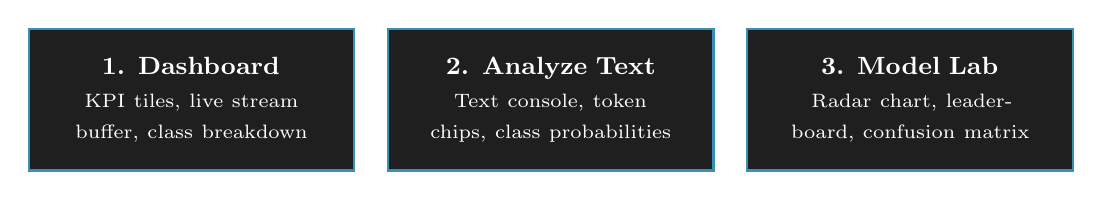
\begin{tikzpicture}[
    node distance=0.4cm,
    screen/.style={rectangle, draw=cyan!70!black, fill=black!88, thick, text=white,
                   text width=3.9cm, align=center, minimum height=1.8cm, font=\small}
]
\node[screen] (s1) {\textbf{1. Dashboard}\\[1pt]\scriptsize KPI tiles, live stream buffer, class breakdown};
\node[screen, right=of s1] (s2) {\textbf{2. Analyze Text}\\[1pt]\scriptsize Text console, token chips, class probabilities};
\node[screen, right=of s2] (s3) {\textbf{3. Model Lab}\\[1pt]\scriptsize Radar chart, leaderboard, confusion matrix};
\end{tikzpicture}
\caption{The three main views of the web platform.}
\label{fig:frontend_views}
\end{figure}

\begin{enumerate}
    \item \textbf{Dashboard (\texttt{/}).} KPI tiles (e.g.\ 15,847 streams processed, 91.6\% accuracy, 12\,ms latency, 73\% Hinglish density), a live event buffer with sentiment badges, and language-distribution charts.
    \item \textbf{Analyze Text (\texttt{/analyze}).} A high-contrast text editor, sample prompts, token-level attribution chips, class-probability bars and a session log.
    \item \textbf{Model Lab (\texttt{/models})}. A banner for the production champion (BiLSTM+Conv1D), the full leaderboard, a multi-axis radar chart and an interactive $3\times3$ confusion matrix.
\end{enumerate}

\begin{table}[htbp]
\centering
\small
\begin{tabular}{ll}
\toprule
\textbf{Design element} & \textbf{Value} \\
\midrule
Background canvas & Obsidian, \texttt{\#090d16} \\
Highlight colour  & Electric cyan, \texttt{\#4cd7f6} \\
Editor text       & \texttt{\#000000} on a light input area \\
Headline font     & Space Grotesk \\
Data font         & Geist Mono \\
Corner radius     & 0\,px (sharp edges) \\
\bottomrule
\end{tabular}
\caption{Stitch design foundations used in the interface.}
\end{table}

% =====================================================================
\section{Reproducibility}
% =====================================================================

\begin{itemize}
    \item \textbf{Fixed seed:} all experiments use random seed $42$.
    \item \textbf{Train-only fitting:} every learned component is fitted on the training split only (Section~2.2).
    \item \textbf{Saved preprocessing:} \texttt{data/processed/preprocessor.json} guarantees that serving applies exactly the same cleaning as training.
    \item \textbf{Checksum manifests:} \texttt{H1\_MANIFEST.json} and \texttt{H2\_MANIFEST.json} verify files between stages.
    \item \textbf{Open data contracts:} the REST/JSON interface and file schemas are fixed, so the backend and frontend can evolve independently.
\end{itemize}

\begin{table}[htbp]
\centering
\small
\begin{tabular}{ll}
\toprule
\textbf{Path} & \textbf{Contents} \\
\midrule
\texttt{src/preprocess.py} & Cleaning and normalisation pipeline \\
\texttt{src/models.py}     & PyTorch model definitions \\
\texttt{data/processed/}   & Processed splits and \texttt{preprocessor.json} \\
\texttt{backend/main.py}   & FastAPI inference service \\
\texttt{frontend/}         & React + TypeScript dashboard \\
\texttt{results.csv}       & Benchmark results used by the dashboard \\
\bottomrule
\end{tabular}
\caption{Main project components.}
\end{table}

% =====================================================================
\section{Limitations and Future Work}
% =====================================================================

\subsection{Limitations}
\begin{itemize}
    \item Results are on the \textbf{validation} split with a \textbf{single seed}; small differences between the top models are not statistically established.
    \item The spelling table currently covers only a few variants (e.g.\ \textit{nahi}), so many spellings rely on FastText alone.
    \item The error analysis is manual and based on a limited sample.
\end{itemize}

\subsection{Future Work}
\begin{itemize}
    \item Fine-tune multilingual transformers (HingBERT, MuRIL, XLM-RoBERTa) using parameter-efficient methods such as LoRA.
    \item Add attention or gradient-based saliency to the dashboard's token inspector to show which words drive each prediction.
    \item Support live streaming input over WebSockets from public social media feeds.
    \item Repeat experiments over several seeds and report confidence intervals.
\end{itemize}

% =====================================================================
\section{Conclusion}
% =====================================================================

We presented HinglishPulse, a complete sentiment analysis system for code-mixed Hinglish text. Starting from the SemEval-2020 Task 9 data, we built strict data contracts, a dialect-aware normalisation pipeline and FastText subword features, and compared five models. The hybrid BiLSTM+Conv1D model achieved the best validation result, a Macro F1 of \textbf{91.64\%} (accuracy 91.57\%), clearly ahead of the 87.12\% Macro F1 of the classical baseline. We then deployed it through a FastAPI service and a React + TypeScript dashboard, closing the gap between a research experiment and a working application.

% =====================================================================
% TODO (authors): please verify the bibliographic details below (authors, titles,
% page numbers) against the official ACL Anthology entries before submission.
\begin{thebibliography}{99}
\bibitem{patwa2020semeval}
P.~Patwa, G.~Aguilar, S.~Kar, S.~Pandey, S.~Rieser, B.~Gamb{\"a}ck, T.~Chakraborty, P.~Fung, and A.~Das,
``SemEval-2020 Task 9: Overview of Sentiment Analysis of Code-Mixed Social Media Text,''
in \textit{Proceedings of the 14th International Workshop on Semantic Evaluation}, pp.~241--260, 2020.

\bibitem{singh2020nits}
N.~Singh and D.~Ghosh,
``NITS-Hinglish-SentiMix at SemEval-2020 Task 9: Sentiment Analysis for Code-Mixed Social Media Text using an Ensemble of BiLSTM and Convolutional Neural Networks,''
in \textit{Proceedings of the 14th International Workshop on Semantic Evaluation}, pp.~1102--1108, 2020.

\bibitem{bojanowski2017enriching}
P.~Bojanowski, E.~Grave, A.~Joulin, and T.~Mikolov,
``Enriching Word Vectors with Subword Information,''
\textit{Transactions of the Association for Computational Linguistics}, vol.~5, pp.~135--146, 2017.

\bibitem{kim2014convolutional}
Y.~Kim,
``Convolutional Neural Networks for Sentence Classification,''
in \textit{Proceedings of the 2014 Conference on Empirical Methods in Natural Language Processing (EMNLP)}, pp.~1746--1751, 2014.
\end{thebibliography}

\end{document}
